\documentclass[letterpaper, 11pt]{article}
%\usepackage[round]{natbib}

\usepackage{mathtools}
\usepackage{setspace} 
\usepackage{dsfont}
\usepackage{amsfonts}
\usepackage{amsmath}
\usepackage{subcaption}
\usepackage{paralist}
%\usepackage{subfig}
\usepackage{times}
\usepackage{latexsym}
\usepackage{graphicx}
\usepackage[T1]{fontenc}
\usepackage{tikz}
\usepackage{url}
\usepackage{pgfplotstable}
\usepackage{titlesec}
\usepackage{color}
\usepackage{lipsum,adjustbox}
\usepackage[font={small}]{caption}
\usetikzlibrary{positioning}
\usepackage{bbm}
\usepackage{booktabs}

\makeatletter
\newcommand{\@BIBLABEL}{\@emptybiblabel}
\newcommand{\@emptybiblabel}[1]{}
%\makeatother
\usepackage[hidelinks]{hyperref}


\usepackage{naaclhlt2018}
\graphicspath{{./plots/}}
\newcommand{\com}[1]{}
%\newcommand{\oa\part{title}}[1]{}
%\newcommand{\lc}[1]{}
\newcommand{\oa}[1]{\footnote{\color{red}OA: #1}}
\newcommand{\oamod}[1]{{\color{red}#1}}
\newcommand{\lc}[1]{\footnote{\color{blue}LC: #1}}
\newcommand{\lcmod}[1]{{\color{blue}#1}}

\newenvironment{myequation}{
  \vspace{-1em}
 \begin{equation}
}{
 \end{equation}
 \vspace{-1.2em}
}
\newenvironment{myequation*}{
	\vspace{-1em}
	\begin{equation*}
}{
\end{equation*}
\vspace{-1.2em}
}


\begin{document}

\title{Translation distributions, coverage and conservatism in monolingual translation}
%\author{
%  Leshem Choshen\textsuperscript{1} and Omri Abend\textsuperscript{2} \\
%  \textsuperscript{1}School of Computer Science and Engineering,
%  \textsuperscript{2} Department of Cognitive Sciences \\
%  The Hebrew University of Jerusalem \\
%  \texttt{leshem.choshen@mail.huji.ac.il, oabend@cs.huji.ac.il}\\
%}
\maketitle

\begin{abstract}
  %Evaluation in Grammatical Error Correction (GEC) is generally carried out
  %by comparison to references. Previous work discussed the necessary low
  %  coverage of such protocols given the multitude of different ways to correct a sentence,
  %and proposed 
  %In this paper we discuss the impact of using 
  %discusses the implications of such reference-based evaluation on
  Through the test case of grammatical error correction (GEC) and a replication on \lc{should we mention GED?} simplification we investigate three aspects of monolingual translation: over-conservatism, the distributions of translations and the coverage of evaluation measures. We find that state-of-the-art systems make substantially fewer changes to the source sentences than needed.
  Analyzing the distributions of possible translations for a given sentence, we show that this over-conservatism likely stems from the inability of a handful of reference corrections to account for the full variation of valid corrections for a given sentence. This results in undue penalization of valid corrections, thus disincentivizing GEC systems (henceforth correctors) to make changes.
  We also show that increasing the number of references is a partial remedy, 
  \lc{should that be changed with the split?}and conclude by presenting reference-less measures (RLM) as an alternative, introducing a GEC RLM based on semantic similarity.
  %one by , and the other by using semantic evaluation.
  %Does grammatical error correction systems learn not to learn?
  %We show that state-of-the-art systems are over conservative and are reluctant to correct. We analyze the distributions of
  % corrections showing that a single ungrammatical sentence tends to have hundreds of valid corrections, a problem for
  %current evaluation methods which are based on a reference or two. We suspect it causes correctors to avoid correcting and proceed to analyze the effect of
  %increasing amount of references in the gold standard on different evaluation measures. Discovering that more references are helpful but only to a
  %certain point, we also find that semantic structures are promising as a measure that is not reference based.
\end{abstract}

\section{Introduction}

% Error correction 
% evaluation in error correction and its centrality
% faithfulness to the source meaning is important, and this has been noted but prev work, and evaluation is geared towards it
% gap in evaluation: however, steps taken to ensure conservativeness in fact push towards formal conservativism by their definition (theoretical claim about the measure)
% this may result in systems that make few changes. indeed we find that this is the case (empirical claim about systems)
%
% we pursue two approaches to overcome this bias.
%
% 1. increasing the number of references. this has been proposed before and pursued with m=2, but no assessment of its sufficiency or its added value over m=1 has been made. In order to address this gap we first charachterize the distribution of possible corrections for a sentence. We leverage this characterization to characterize the distribution of the scores as a function of $m$, and consequently assess the biases introduced by taking $m=1,2$ as with previous approaches. 
% We find that taking these values of $m$ drammatically under-estimate the system scores. 
% We back our analysis of these biases with an analysis of the variance of these estimators.
% We analyze the two commonly used scores, the M2 score often used for evalauted, and the accuracy score commonly used in training.
%
% 2. we note that in fact the important factor is semantic conservativism and explore means to directly assess how semantically conservative systems here through the use of semantic annotation. 
% We use the UCCA scheme as a test case, motivated by HUME.
% First question: is it well-defined on learner language. it is.
% Second question: are corrections in fact semantically conservate? to show that, we need to verify that the corrections make few (if any) semantic changes. our results indicate that this is the case: we show that the corrections are similar in (UCCA) structure to the source.
%
% conclusion (not in intro): we tried to use semantic similarity to improve systems.
% this is difficult due to semantic conservatism. we expect this will be in issue once evaluation is improved.
% future work.
% also future work: use multiple references in training (did people do that?)
%
% sections:
% 1. Introduction
% 2. Formal conservativism in GEC
% 3. First approach: Multiple References
% 3.1. A Distribution of Corrections
% 3.2. Scores (M2, accuracy index, accuracy exact)
% 3.3. Data
% 3.4. Bias of the Scores (setup + results)
% 3.5. Variance of the Scores (setup + results)
% 4. Second approach: Semantic Similarity
% 4.1. Semantic Annotation of Learner Language (prev work)
% 4.2. UCCA Scheme (see HUME)
% 4.3. Similarity Measures (including prev work of elior)
% 4.4. Empirical Validation: IAA, semantic conservativism vs. gold std
% 5. Conclusion
%
% is a challenging research field, which interfaces with many
%other areas of linguistics and NLP. The field
Grammatical Error Correction (GEC) is receiving considerable
interest recently, notably through the GEC-HOO \cite{dale2011helping,dale2012hoo} and
CoNLL shared tasks \cite{kao2013conll,ng2014conll}.
Within GEC, considerable effort has been placed on evaluation
\cite{tetreault2008native,madnani2011they,felice2015towards,napoles2015ground},
a notoriously difficult challenge, in part due to the many valid corrections a learner's language (LL) sentence may have \cite{chodorow2012problems}. Thus, we chose to take it as the main test case for this paper, in \ref{sec:simplification} we follow the same procedure, with less details over the field of simplification suggesting that our findings are general and apply to various monolingual translation tasks.

An important criterion in the evaluation of correctors is their faithfulness to the meaning of the source. In fact, it has been argued that many would prefer a somewhat cumbersome or even an occasionally ungrammatical correction over one that alters the meaning of the source \cite{brockett2006correcting}.
Consequently, annotators are often instructed to be conservative when compiling gold standard corrections for the task
(e.g., in the Treebank of Learner English \cite{nicholls2003cambridge}).
There were different attempts in evaluation procedures to formally capture this precision/recall asymmetry such as the standardized use of $F_{0.5}$ over $F_{1}$ \cite{dahlmeier2012better} and the choices of weights in I-measure \cite{felice2015towards}.

However, penalizing over-correction more harshly than under-correction during development and training, may lead to reluctance of correctors to make any changes (henceforth, {\it over-conservatism}).
Using only one or two reference corrections, the common practice in GEC, compounds this problem, as correctors are not only harshly penalized for making incorrect changes, but are often penalized for making {\bf correct} changes not found in the reference.

Indeed, we show that current state of the art systems present over-conservatism.
Evaluating the output of 15 recent correctors, we find they all
substantially under-predict corrections relative to the already conservative gold standard
(\S\ref{sec:formal_conservatism}). 
As the gap in the prevalence of corrections between references and correctors' output is often an order of magnitude large, this effect is unlikely to be desirable. See discussion in \S\ref{sec:increase-reference}.

We first assess the effect of increasing the number of references, denoted $\mathcal{M}$, on the undue penalization of valid corrections (\S \ref{sec:increase-reference}).
We start by estimating the number and frequency distribution of the valid corrections per sentence, arriving at an estimate of over \textbf{1000} corrections for short sentences.
We then consider two representative reference-based measures (henceforth, {\it RBMs}) for
assessing the validity of a proposed correction relative to a set of references, 
and characterize the distribution of their scores as a function of $\mathcal{M}$. 
Our results show that both measures substantially under-estimate the true performance of
the correctors. Moreover, they show that increasing $\mathcal{M}$ only partially addresses the incurred bias, as both RBMs' assessment almost triple with the increasing $\mathcal{M}$ but it plateaus for values of 10--20, reaching about $60\%$.
%indicating that a prohibitively large $\mathcal{M}$ may be required for reliable estimation.


\lc{I think that may be be moved or removed from the introduction:
	Our findings echo the results of \newcite{bryant2015far}, who study the effect of $\mathcal{M}$ on $F$-score, but the additional results in this paper suggests that their solution is still lacking. 
	%who study the effect of $\mathcal{M}$ on $F$-score, the most commonly used measure for GEC.
	Their work focused on obtaining a more reliable estimate of correctors' performance and proposed to do so by normalizing corrector's estimated performance with the performance of a human corrector.
%Our findings echo the results of \newcite{bryant2015far}, who study the effect of $\mathcal{M}$ on $F$-score, the most commonly used measure for GEC. Their work focused on obtaining a more reliable estimate of correctors' performance and proposed to do so by normalizing corrector's estimated performance with the performance of a human corrector.
However, while such normalization may yield more realistic performance estimates,
it has no effect on the training and tuning of correctors. Moreover, we show that it already yields above perfect score for a system that hardly corrects.
}

We then turn our gaze to simplification, showing that over-conservatism, vast number of simplifications\lc{perhaps something more exact when we have data} and low coverage are all just as relevant.

\lc{never seen self linking, is this how it should be done?}
We conclude by proposing semantic RLMs as an alternative. Specifically, we introduce in another paper sent to this conference GEC RLM to assess the extent to which
a correction faithfully represents the semantics of the source, by their semantic structures similarity(\S \ref{sec:Semantics}).
This approach can be combined with RLM based on grammatical error detection(GED), as proposed by \newcite{napoles-sakaguchi-tetreault:2016:EMNLP2016}.
%Our experiments support the feasibility of the proposed approach,by showing that (1) semantic structural annotation can be consistently and automatically applied to LL, (2) that the proposed measure is less prone to unduly penalize valid corrections and (3) that the measure does penalize corrections that alter the semantic structure significantly.

%
%
%We define a measure, using the UCCA scheme \cite{abend2013universal} as a
%test case, motivated by its recent use for machine translation
%evaluation \cite{birch2016hume}.
%We annotate a section of the NUCLE parallel corpus \cite{dahlmeier2013building},
%
%The two approaches address the insufficiency of using too few references from
%complementary angles. The first attempts to cover more of the probability
%mass of valid corrections by taking a larger $\mathcal{M}$, 
%while the second uses semantic instead of string similarity, in order
%to abstract away from some of the formal variation between different valid corrections.
%
%%%%%%%%%%%%%%%%%%%%%%%%%%%%%%%%%%%%%%%%%%%%%%%%%%%%%%%%%%%%%%%%%%%%%%%%%%%%%%
\section{Over-Conservativism in GEC Systems}\label{sec:formal_conservatism}
%The field of GEC was always thriving or conservatism in its corrections, with the prominent example of using
%$F_{0.5}$ emphasizing precision over recall(\cite{ng2014conll}). we wish to highlight the problem that
%arises from pursuing this conservatism as done today.
%Then, we wished to be conservative, and we achieved that, why shouldn't we rejoice just yet? Theoretically, we might be progressing towards not correcting at all, instead of progressing towards correcting more accurately. 
%
%Manual analysis showed excessive formal conservatism and under correction.
%Albeit important, manual analysis is not enough and we aimed for generating some quantitative measures. 
%
%We demonstrate that current correctors
%suffer from over-conservatism: they tend to make too few changes to the source, relative to human correctors.
%{ \color{red} This is likely an indication of some hidden, cross-systems, widely spread  bias.}

\paragraph{Notation.}
We assume each LL sentence $x$ has a set of valid corrections $Correct_x$,
and a discrete distribution $\mathcal{D}_x$ over them, where $P_{\mathcal{D}_x}(y)$
for $y \in Correct_x$ is the probability a human annotator would correct $x$ as $y$.

Let $X=x_{1}\ldots x_{N}$ be the evaluated set of source LL sentences and denote $\mathcal{D}_{i}\coloneqq \mathcal{D}_{x_i}$. Each $x_{i}$ is independently sampled from some distribution $\mathcal{L}$ over LL sentences 
and each is paired with $\mathcal{M}$ corrections $Y_i = \left\{y_{i}^{1},\ldots, y_{i}^{\mathcal{M}}\right\}$,
which are independently sampled from $\mathcal{D}_{i}$. Our analysis assumes a fixed $M$. Generalizing to sentence-dependent $M$ is straightforward.
We define the {\it coverage} of a reference set $Y_i$ of size $\mathcal{M}$ for a sentence $x_i$ to be $P_{y \sim \mathcal{D}_i}(y \in Y_i)$.

A corrector $C$ is a function from LL sentences to proposed corrections (strings).
An assessment measure is a function $f\colon X\bigtimes Y\bigtimes C\to \mathbb{R}$. We use the term ``true measure'' to refer to a measure's output where the references include all possible corrections, i.e., $\forall i\colon Y_i=Correct_i$.

\paragraph{Experimental Setup.}\label{par:experimental_setup}
We conduct all experiments on the NUCLE test dataset \cite{dahlmeier2013building},
a parallel corpus of LL essays and their corrected versions,
which is the de facto standard in GEC.
The corpus contains 1414 essays in LL and 50 test essays, each of about 500 words.

We evaluate all participating systems in CoNLL 2014 shared task,
in addition to three of the best performing systems on this dataset, a hybrid corrector \cite{rozovskaya2016grammatical}, a phrase based machine translation(MT) \cite{junczysdowmunt-grundkiewicz:2016:EMNLP2016} and a neural network based corrector \cite{xie2016neural}.
See Appendix \ref{ap:abbr} for system names and abbreviations. %All systems were trained and tested on the NUCLE corpus.

We compare the prevalence of changes made to the source by the correctors,
relative to their prevalence in the NUCLE references (one annotator was arbitrarily selected for the figures). \newcite{bryant2015far} noticed that the NUCLE references are more conservative than the ones they collected, which implies that our results may even underestimate the level of conservatism relative to other references.
\lc{it seems so technical I wonder if it is still relevant} To evaluate meaningful changes, all non-alphanumeric characters were excluded, both within tokens or as tokens of their own.

\paragraph{Measures of Conservatism.}
We consider three types of divergences between the source and the reference.
First, we measure the extent to which \emph{words} were changed: altered, deleted or added.
To do so, we compute word alignment between the source and the reference, casting it
as a weighted bipartite matching problem. Edge weights are assigned to be the edit distances between the tokens.
We note that aligning words in GEC is much simpler than in MT,
as most of the words are unchanged, deleted fully, added, or changed slightly.
Following word alignment, we define {\sc WordChange}
as the number of unaligned words and aligned words that were changed in any way.

Second, we quantify word \emph{order} differences using
Spearman's $\rho$ between the order of the words in the source sentence
and the order of their corresponding-aligned words in the correction.
$\rho=0$ where the word order is uncorrelated, and $\rho=1$ where the orders exactly match. We report the average $\rho$ over all source sentences pairs. 

Third, we report how many source sentences were split and how many concatenated by the reference and the correctors.

\begin{figure}
	\vspace{-0.8cm}
  \centering
  \begin{subfigure}[]{0.35\textwidth}
    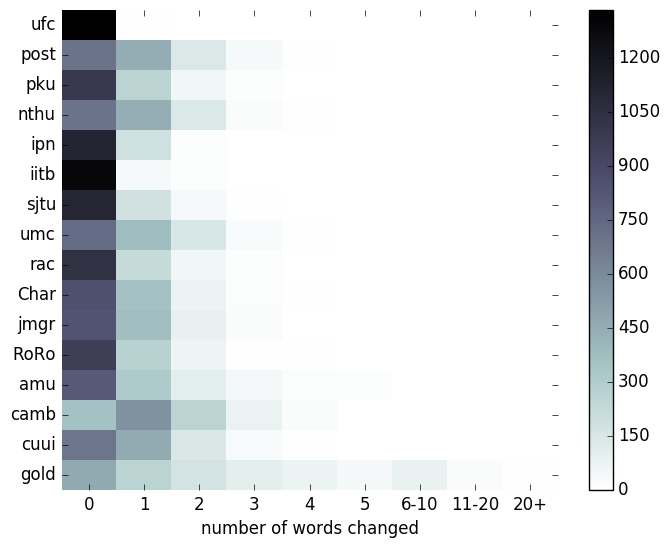
\includegraphics[width = \textwidth]{words_differences_heat}
  \end{subfigure}
  \begin{subfigure}[]{0.35\textwidth}
    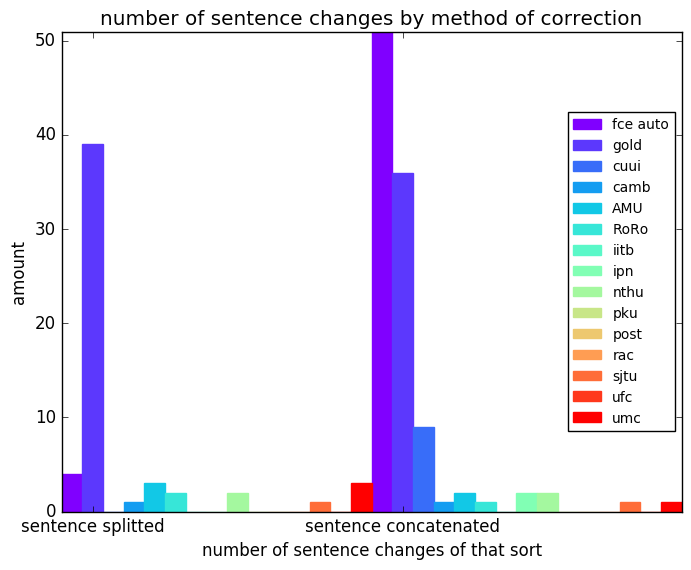
\includegraphics[width = \textwidth]{aligned}
  \end{subfigure}
  \begin{subfigure}[]{0.35\textwidth}
    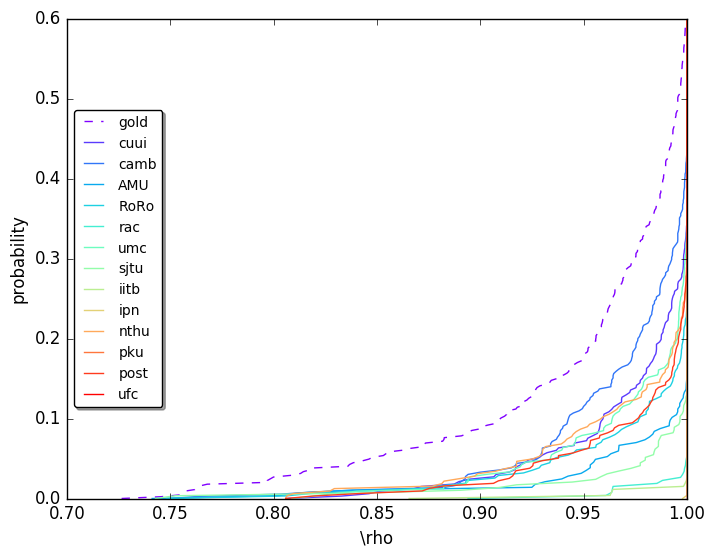
\includegraphics[width = \textwidth]{spearman_ecdf}
  \end{subfigure}
  \caption{\label{fig:over-conservatism}
    The prevalence of changes correctors' outputs and in the NUCLE reference.
    The top figure presents the amount of sentences (heat) for each amount of word changes
    (x-axis; measured by {\sc WordChange}) done by the outputs and the reference (y-axis).
    The middle figure presents the counts of source sentences (y-axis) concatenated (right bars) or split (left bars) by the references (striped column) and the outputs (colored columns).
    The bottom figure presents the percentage of sentence pairs (y-axis) where the
    Spearman $\rho$ values do not exceed a certain threshold (x-axis).
    See Appendix \ref{ap:abbr} for a legend of the correctors.
    Under all measures, the gold standard references make substantially more changes to the source sentences than any of the correctors,in some cases an order of magnitude more.
  }
\vspace{-0.8cm}
\end{figure}

\paragraph{Results.}
% presents the outcome of the three measures. 
%In \ref{fig:split} the amount of sentences each corrector has done is presented. In \ref{fig:words_changed} the accumulated sum of sentences by the words changed in each sentence of each of the correctors is presented. In \ref{fig:rho} the cumulative probability distribution of rho values out of all the sentences.
Results (Figure \ref{fig:over-conservatism}) show that reference corrections change considerably more source sentences than any of the correctors, and within each changed sentence both change and reorder more words, often an order of magnitude more. For example, there are  36 reference sentences with 6 word changes, where the most sentences with 6 word changes by any corrector is 5.
Similar amount of correction is observed on the references of the TreeBank of Learner English \cite{yannakoudakis2011new}.
%While $89.6\%$ of NUCLE sentences need corrections,
%The prevalence of FCE consists only of ungrammatical sentences.
%As expected, FCE is a bit less conservative than NUCLE by our measures.
%
%
%%%%%%%%%%%%%%%%%%%%%%%%%%%%%%%%%%%%%%%%%%%%%%%%%%%%%%%%%%%%%%%%%%%%%%%%%%%%%%%%%%%%%
\vspace{-.1cm}
\section{Multi-Reference Measures}\label{sec:increase-reference}
%
In this section we argue that the observed over-conservatism of correctors likely stems
from them being developed to optimize RBMs that suffer from low-coverage.
We present a motivating analysis of the relation between low-coverage and over-conservatism (\S \ref{subsec:motivating_analysis}). We then continue with an assessment of the distribution of corrections for a given sentence (\S \ref{subsec:corrections_distribution})
and the effect of $\mathcal{M}$ on commonly used\lc{commonly used or used in training and validation?} RBMs (\S \ref{subsec:Assessment-values}).
We discuss our results' implications, concluding that RBMs may only partially address over-conservatism (\S \ref{subsec:mult_discussion}).
%
\vspace{-.2cm}
\subsection{Motivating Analysis}\label{subsec:motivating_analysis}
%
The relation between coverage and over-conservatism requires some explanation.
We abstract away from the details of the training procedure and assume that correctors attempt to maximize an objective function, over some training or development data, and assume for simplicity of the argument that improvement is achieved by iterating over the samples, as with the Perceptron algorithm.

Assume the corrector is faced with a phrase which it predicts to be ungrammatical. Assume $p_{detect}$ is the probability that this prediction is correct.
Assume $p_{correct}$ is the probability it is able to predict
a valid correction for this phrase (including correctly identifying it as erroneous).
Finally, assume the corrector is evaluated
against $\mathcal{M}$ references for which the coverage is $p_{coverage}$,
namely the probability that
a valid correction will be found among $\mathcal{M}$ randomly sampled references.

We will now assume that the corrector may either choose to correct with the correction it finds the most likely or not at all. If it chose not to correct, its probability of being rewarded (i.e., its output is in the reference set $Y$) is $(1-p_{detect})$. Otherwise, its probability
of being rewarded is $p_{correct} \cdot p_{coverage}$.
A corrector is disincentivized from altering the phrase in cases where:

\vspace{.1cm}
\begin{small}
\begin{myequation}
  \label{eq:reward}
  p_{correct} \cdot p_{coverage} < 1-p_{detect} 
\end{myequation}
\vspace{-.1cm}
\end{small}


We expect Condition (\ref{eq:reward}) to frequently hold in cases that
require non-trivial changes, which are characterized both by low $p_{coverage}$ (as non-trivial
changes can often be made in numerous ways), and by lower performance by the corrector.

Moreover, asymmetric measures (e.g., $F_{0.5}$) penalize invalidly correcting more
harshly than not correcting an ungrammatical sentence.
In these cases, Condition (\ref{eq:reward}) should be rephrased as

\begin{small}
	\vspace{-.1cm}
  \begin{myequation*}
    p_{correct} \cdot p_{coverage} - \left(1-p_{correct}p_{coverage}\right) \alpha < 1-p_{detect} 
  \end{myequation*}
  \vspace{-.1cm}
\end{small}

where $\alpha$ is the ratio between the penalty for introducing a wrong correction and the reward for a valid correction. The condition is even more likely to hold in these cases.
Validating this analysis empirically, we conduct an experiment to determine whether increasing
the number of references in training indeed reduces conservatism. There is no multiple-reference
corpus available which is large enough for re-training a corrector. Hence, we take an oracle reranking approach
as a simulation, and test whether the availability of increasingly more training references reduces its conservativeness.
Concretely, given a set of sentences, each paired with $\mathcal{M}$ references; a measure and a corrector's $k$-best list, we define an oracle re-ranker that selects for each sentence the highest scoring correction.
As a test case, we use the RoRo system, with $k=100$, and apply it to the 
largest available LL corpus which is paired with a substantial amount of GEC references,
namely the NUCLE-test corpus. Using the common $F$-score as an evaluation measure. 
We examine the conservativeness of the oracle reranker for different $\mathcal{M}$ values, averaging over 1312 samples of $\mathcal{M}$ references from the available set of $\mathcal{M}=12$ \cite{bryant2015far}.

Our results show that word changes increase with $\mathcal{M}$ (Figure \ref{fig:reranking_word_change}). No significant difference is found in word order.
%\footnote{As we only rerank individual sentences,
%  there is clearly no change in the number of sentences split or concatenated.}
This indicates that conservatism is indeed related to the number of references available
to the learner.

We do not see a reason why this reduction in conservatism may result from the setup itself. In fact, oracle reranking will not show this tendency if even one of our assumptions does not hold. For simplicity, lets assume we only consider a specific error and collapse the corrections in the $k$-best list to three: $S$ keeping the source untouched, $VC \subset Correct$ the valid corrections and invalid ones. Then, aided by table \ref{ta:oracle_expected_results} we see that if over-conservatism is due to systems' lack of ability, if most choices not to correct are valid and hence probable to be found in some of the references or if coverage is not a problem, then we would expect no conservatism reduction in the experiment. 
%
\begin{table}[h]
	\vspace{-0.5cm}
	\centering
	\small
	\singlespacing
	\begin{tabular}{cc|cc}
		& No VC & \multicolumn{2}{c}{VC exist in k-best list}                                                                                \\
		& Any S           & S  Correct                                                                              & S Erroneous \\ \hline
		\multicolumn{1}{c|}{Small $\mathcal{M}$} & 1          & \begin{tabular}[c]{@{}c@{}}$P\left(S, \neg VC\right) +$\\  $0.5 P\left(S, VC\right)$\end{tabular} & $P\left(VC\right)$    \\
		\multicolumn{1}{c|}{Large $\mathcal{M}$} & 1          & 0.5                                                                                          & 0                  \\ \hline
		\multicolumn{1}{c|}{Expected}            & No change  & \begin{tabular}[c]{@{}c@{}} Undefined\end{tabular}        & More changes 
	\end{tabular}
	\caption{The expected results under different assumptions concerning the ability of correctors to correct, the need for correcting most of the errors, and the probability for high coverage with small $\mathcal{M}$. The values represent the probabilities keeping the source. $P$ is the probability to be in $Y$. \label{ta:oracle_expected_results}}
	\vspace{-0.6cm}
\end{table}
%
\begin{figure}
	\vspace{-1em}
	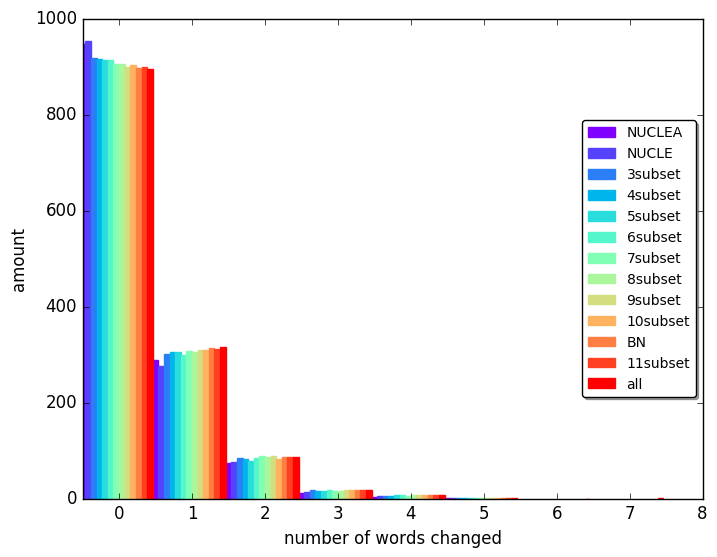
\includegraphics[width=8cm]{words_differences_hist_reranking}
	\caption{The amount of sentences (y-axis) with a given number of words changed (x-axis), following oracle reranking with different $\mathcal{M}$ values (column colors). All references are randomly sampled except BN column that contains \newcite{bryant2015far} 10 references.
		In conclusion, tuning against additional references indeed reduces conservatism.
		\label{fig:reranking_word_change}
        }
	\vspace{-0.5cm}
\end{figure}
%
 \subsection{Data}
%
%Our analysis assumes that we have a reliable estimate for the distribution of corrections
$\mathcal{D}_x$ of the source sentences we evaluate.
The experiments in the following section are run on a random sample of 52 sentences with a maximum length of 15 from the NUCLE test data.
Through the length restriction we avoid introducing too many independent errors that may drastically increase the number of annotation variants (as every combination of corrections for these errors is possible), thus resulting in an unreliable estimation for $\mathcal{D}_x$.
Sentences with less than 6 words were discarded, as they were mostly a result of sentence segmentation errors.

Proven to be effective in GEC \cite{madnani2011they} and related tasks such as MT \cite{zaidan2011crowdsourcing, post2012constructing}, we use crowdsourcing for obtaining a sample from $\mathcal{D}_x$. Specifically, for each of the 52 source sentences, we elicited 50 corrections from Amazon Mechanical Turk workers.
%allowing for a reliable estimation of the distributions.
Aiming to judge grammaticality rather than fluency, we instructed the workers to
correct only when necessary, not for styling.
4 sentences required no correction according to almost half the workers and were hence discarded.
%
\subsection{Estimating Corrections' Distribution}\label{subsec:corrections_distribution}
%
We begin by estimating $\mathcal{D}_x$ for each sentence, using the crowdsourced corrections.
We use {\sc UnseenEst} \cite{zou2015quantifying}, a non-parametric algorithm to
estimate a discrete distribution in which the individual values do not matter, only the probability of each value. {\sc UnseenEst} aims to minimize the ``earthmover distance'', between the estimated histogram and the histogram of the distribution. Intuitively, if histograms are piles of dirt, minimizing the amount of dirt moved times the distance by which it was moved.\footnote{An implementation of {\sc UnseenEst} can be found in <to be disclosed upon publication>\com{\href{https://github.com/borgr/unseenest}}} 
{\sc UnseenEst} was originally developed and thoroughly tested for assessing how many
variants a gene might have, including undiscovered ones, and their relative frequencies.
This is a similar setting to the one tackled here.
Our manual tests of {\sc UnseenEst} with small artificially created datasets
showed satisfactory results.\footnote{All data we collected, along with the estimated
  distributions can be found in <to be disclosed upon publication>}

According to the estimates, most LL sentences have a large number of
infrequent corrections accounting for the bulk of the probability mass
and a rather small number of frequent corrections.
%The estimated distributions tend to have steps, with many corrections with the same (low) frequency.
Table \ref{tab:corrections_dist} presents the mean number of different corrections with frequency at least $\gamma$ (for different $\gamma$ values), and their total probability mass.
For instance, 74.34 corrections account for 75\% of the total probability mass of the corrections, each occurring with a frequency of 0.1\% or higher.

\begin{table}[h!]
	\vspace{-0.5cm}
  \centering
  \small
  \singlespacing
  \begin{tabular}{c|c|c|c|c|}
    %\cline{2-5} 
    & \multicolumn{4}{c|}{Frequency Threshold ($\gamma$)}\\ 
    %\cline{2-5} 
    & \multicolumn{1}{c}{0} & \multicolumn{1}{c}{0.001} & \multicolumn{1}{c}{0.01} & \multicolumn{1}{c|}{0.1}
    \\
    \hline
    Variants & 1351.24 & 74.34 & 8.72 & 1.35
    \\
    Mass & 1 & 0.75 & 0.58 & 0.37\\
    \hline
  \end{tabular}
  \caption{\label{tab:corrections_dist}
    Estimating the distribution of corrections $\mathcal{D}_x$.
    The table presents the mean number of corrections per sentence with probability of more than
    $\gamma$ (top row), as well as their total probability mass (bottom row).
  }
  \vspace{-0.3cm}
\end{table}

The overwhelming number of rare corrections raises the question of whether these can be regarded as noise.
To test this we conducted another crowdsourcing experiment, where 3 annotators were asked to judge whether a correction produced in the first experiment, is indeed a valid correction.
Figure \ref{fig:validity_judgements} presents the frequency in which annotators judged a correction to be valid, where corrections are grouped by the number of times they appear in the data.

Results show that the empirical frequency of a correction has little effect on how often it was deemed valid, where even the rarest corrections were judged valid 78\% of the times.
\lc{perhaps move to the appendix}
\begin{figure}[h!]
	\vspace{-.3cm}
	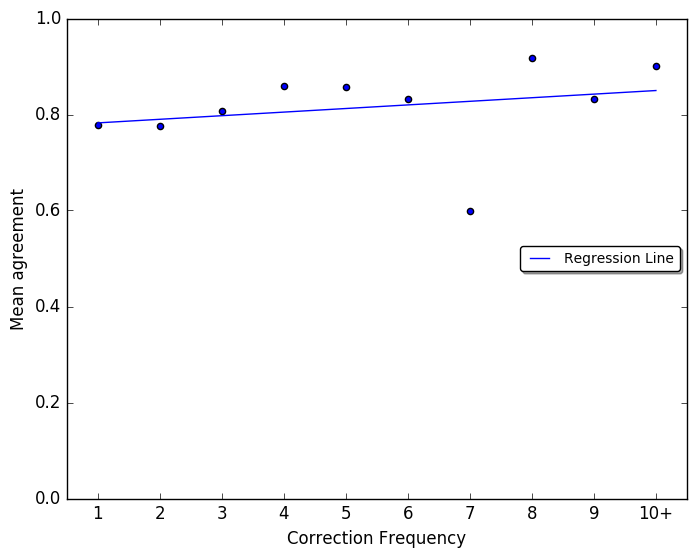
\includegraphics[width=8cm]{IAA_confirmation_frequency}
	\caption{The mean frequency ($y$-axis) in which a correction that was produced
          a given number of times ($x$-axis), was judged to be valid.
	} \label{fig:validity_judgements}
	\vspace{-0.3cm}
\end{figure}

\subsection{Under-estimation as a function of $\mathcal{M}$} \label{subsec:Assessment-values}
In the previous section we presented an empirical assessment of the corrections distribution of a sentence. We turn to estimating the resulting bias, i.e., the under-estimation of RBMs, for different $\mathcal{M}$ values. 
We discuss two similarity measures: sentence-level accuracy
(or ``Exact Match'') and the GEC $F$-score.

\paragraph{Sentence-level Accuracy.}
Sentence-level accuracy is the percentage of corrections that
exactly match one of the references.
Accuracy is a basic, interpretable measure, used in GEC by, e.g., \newcite{rozovskaya2010annotating}.
It is also closely related to the 0-1 loss function commonly used
for training statistical correctors \cite{chodorow2012problems,rozovskaya2013joint}. 

Formally, given test sentences $X=\{x_1,\ldots,x_N\}$,
their references $Y_1,\ldots,Y_N$, and a corrector $C$,
we define $C$'s accuracy to be

\begin{small}
\vspace{-0.2cm}
  \centering
  \begin{myequation}\label{eq:acc_def}
    Acc\left(C;X,Y\right) = \frac{1}{N} \sum_{i=1}^N \mathds{1}_{C(x_i) \in Y_i}.
  \end{myequation}
\end{small}

Note that $C$'s accuracy is, in fact, an estimate of $C$'s {\it true accuracy}, the probability to produce a valid correction for a sentence. Formally:
\lc{read until here}
 \begin{small}
   \centering
   \vspace{-0.2cm}
   \begin{myequation*}
     TrueAcc\left(C\right) = P_{x\sim{L}}\left(C\left(x\right)\in Correct_x\right).
   \end{myequation*}
   \vspace{-0.15cm}
 \end{small}
%
%We estimate $C$s quality by sampling a set of source sentences
%$x_1,\ldots,x_N \sim \mathcal{L}$, and evaluate the quality of $C(x_1),\ldots,C(x_N)$ relative
%to the source. 

The bias of $Acc\left(C;X,Y\right)$ for a sample of $N$ sentences, each paired with $\mathcal{M}$ references
is then

\vspace{-0.6cm}
\begin{small}
  \centering
  \begin{flalign}
    &TrueAcc\left(C\right) - \mathbb{E}_{X,Y}\left[Acc\left(C;X,Y\right)\right] = &\\
    &TrueAcc\left(C\right) - P\left(C\left(x\right) \in Y\right)  = &\\
    &P\left(C\left(x\right) \in Correct_x\right)  \cdot &\\
    &\label{eq:bias} \left(1 - P\left(C\left(x\right) \in Y \vert C\left(x\right) \in Correct_x\right) \right) &
  \end{flalign}
\end{small}
\vspace{-1.5em}

We observe that the bias, denoted $b_\mathcal{M}$, is not affected by $N$, only by $\mathcal{M}$.
As $\mathcal{M}$ grows, $Y$ approximates $Correct_x$ better, and $b_\mathcal{M}$ tends to 0.

In order to gain insight into the evaluation measure and the GEC task
(and not the idiosyncrasies of specific systems), we consider an idealized learner,
which, when correct, produces a valid correction with the same
distribution as a human annotator (i.e., according to $\mathcal{D}_x$).
Formally, we assume that, if $C(x) \in Correct_x$ then $C(x) \sim \mathcal{D}_x$.
Hence the bias $b_\mathcal{M}$ (Equation \ref{eq:bias}) can be re-written as

\begin{small}
	\vspace{-0.2cm}
\begin{myequation*}
  \centering
  P(C(x) \in Correct_x) \cdot (1 - P_{Y \sim \mathcal{D}_i^\mathcal{M},y\sim \mathcal{D}_x}(y \in Y)).
\end{myequation*}
\end{small}

We will henceforth assume that $C$ is perfect (i.e., its true accuracy $Pr\left(C(x) \in Correct_x\right)$ is 1).
Note that assuming any other value for $C$'s true accuracy
would simply scale $b_\mathcal{M}$ by that accuracy.
Similarly, assuming only a fraction $p$ of the sentences require correction scales $b_\mathcal{M}$ by $p$.
%
%Denote the bias of a perfect corrector with $b_\mathcal{M}$. To recap:
%\begin{equation*}
%  b_\mathcal{M} = 1 - P_{x \sim L, Y \in \mathcal{D}_x^\mathcal{M}, y \sim \mathcal{D}_x}\left(y \in Y\right)
%\end{equation*}
%
%We turn to estimating $b_\mathcal{M}$ empirically. We note that $Acc(C;X,Y)$
%is a sum of Bernoulli variables (i.e., a Poisson Binomial distribution), 
%with probabilities $p_i = P_{y \sim \mathcal{D}_i}\left(y \in Y_i\right)$.

We estimate $b_\mathcal{M}$ empirically using its empirical mean on our experimental corpus:

\begin{small}
	\vspace{-1em}
  \begin{myequation*}
    \hat{b}_\mathcal{M} = 1 - \frac{1}{N}\sum_{i=1}^N P_{Y \sim \mathcal{D}_i^\mathcal{M}, y \sim \mathcal{D}_i}\left(y \in Y\right).
  \end{myequation*}
\end{small}

Using the {\sc UnseenEst} estimations of $\mathcal{D}_i$, we can compute $\hat{b}_\mathcal{M}$ 
for any size of $Y_i$($=\mathcal{M}$). 
However, as this is highly computationally demanding, we estimate it using
sampling. Specifically, for every $\mathcal{M} = 1,...,20$ and $x_i$, we sample $Y_i$ 1000 times (with replacement), and estimate $P\left(y \in Y_i\right)$ as the covered probability mass $P_{\mathcal{D}_i}\{y: y \in Y_i\}$.

We repeated all our experiments where $Y_i$ is sampled without replacement,
in order to simulate a case where reference corrections are collected by a single
annotator, and are thus not repeated. We find similar trends with a faster increase
in accuracy reaching over $0.47$ with $\mathcal{M}=10$.
%
%The resulting estimates for $p_i$ 
%define the estimate for the distribution of $Acc(C;X,Y)$.
%Given a set of LL sentences $x_1,...,x_N$ and their corresponding references
%$Y_1,...,Y_N$, we define the coverage of the reference set $Y_i$ for the sentence $x_i$ to be
%
%\begin{equation*}
%Cov\left(x_i,Y_i\right)=.
%\end{equation*}
%
%In order to gain insight into the accuracy measure, we need to know something about the distribution from which the given corrector chooses valid corrections. As each corrector might have its own biases, the most appealing choice would be to evaluate a corrector in which this distribution is the same as the one from which corrections for the gold standard are being drawn from. Formally, if $C\left(x_i\right) \in Correct_i$ then $C\left(x_i\right) \sim \mathcal{D}_i$. 
%
%Thus, the second term in Equation \ref{eq:correction-in-gs} is $p_i = \mathbb{E}_{Y_i}[Cov(x_i,Y_i)]$. 
%Therefore $Acc(C;X,Y)$ is distributed as
%a Poisson Binomial random variable (divided by $N$), with probabilities $\{p_i \cdot CP\}_{i=1}^N$. \footnote{A Poisson Binomial random 
%variable is a sum of Bernoulli variables with different success probabilities.} We also assume our corrector is always 
%correct (so $CP=1$), but as noted earlier any other value for $CP$ would only scale the results by $CP$.

\begin{figure}
	\vspace{-1em}
  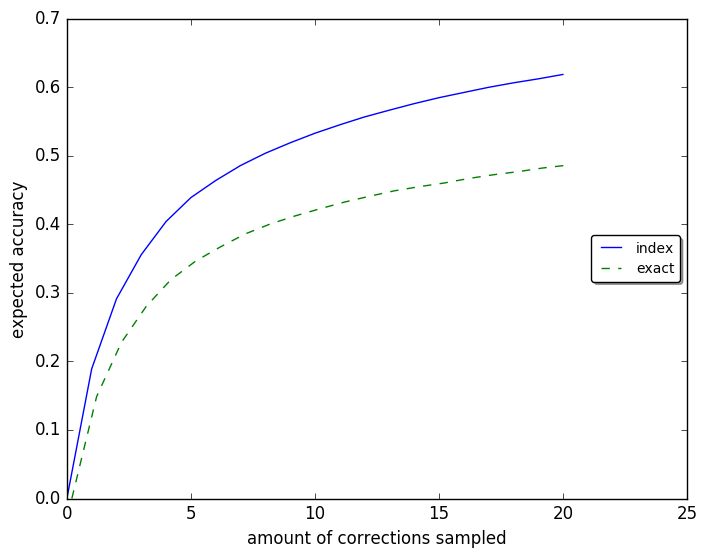
\includegraphics[width=8cm]{noSig_repeat_1000_accuracy}
  \caption{Accuracy and Exact Index Match values for a perfect corrector (y-axis)
    as a function of the number of references $\mathcal{M}$ (x-axis).
    %Each data point is paired with a confidence interval ($p=.95$).     
  } \label{fig:accuracy_vals}
  \vspace{-0.5cm}
\end{figure}

Figure \ref{fig:accuracy_vals} presents the expected accuracy values for our perfect
corrector (i.e., 1-$\hat{b}_\mathcal{M}$) for different  $\mathcal{M}$ values. 
Results show that even for $\mathcal{M}$ values which are much larger than those normally used (e.g., $\mathcal{M}=20$),
the expected accuracy is only about 0.5. As $\mathcal{M}$ increases, the contribution of each additional correction diminishes sharply (the slope is about 0.004 around $\mathcal{M}=20$).

We also experiment with a more relaxed measure, {\it Exact Index Match}, which is only sensitive to the identity of the changed words and not to what they were changed to. 
Formally, two corrections $c$ and $c'$ over a source sentence $x$ match if for their word alignments with the source (computed as above) $a:\{1,...,\left|x\right|\} \rightarrow \{1,...,\left|c\right|,Null\}$
and $a':\{1,...,\left|x\right|\} \rightarrow \{1,...,\left|c'\right|,Null\}$, it holds that $c_{a\left(i\right)} \neq x_{i} \Leftrightarrow c'_{a'\left(i\right)} \neq x_{i}$, where $c_{Null}=c'_{Null}$.

Figure \ref{fig:accuracy_vals} also presents the expected accuracy in this case
for different values of $\mathcal{M}$, which indicate that while scores of a perfect corrector are somewhat higher, still with $\mathcal{M}=10$, it is 0.54.
As Exact Index Match can be interpreted as an accuracy measure for GED, this indicates that GED evaluation suffers from similar difficulties.

The analytic tools we have developed support the computation of the entire distribution of the accuracy, and not only its expected values. From Equation \ref{eq:acc_def} we see that Accuracy has a Poisson Binominal distribution (i.e., it is a sum of independent Bernoulli variables with different success probabilities), whose success probabilities are $P_{y,Y \sim \mathcal{D}_i}(y \in Y)$, which can be computed, as before, using {\sc UnseenEst}'s estimate for $\mathcal{D}_i$. Estimating the density function allows for the straightforward definition of significance tests for the measure, and can be performed efficiently \cite{hong2013computing}.\footnote{An implementation of this and other methods and the estimated density functions will be released upon publication.}

\paragraph{$F$-Score.}
While accuracy is commonly used as a loss function for training GEC systems,
the $F_\alpha$-score is standard when reporting system performance (and consequently in hyper-parameter tuning and development). \lc{Do we really need to elaborate on F score history in GEC?}
Computing $F$-score for GEC is not at all straightforward.
The score is computed in terms of {\it edit} matches between a correction and the references, where edits are sub-string replacements to the source.
The HOO shared task used an earlier version of $F$-score, which required that the proposed corrections include edits explicitly.
Later on, relieving correctors from the need to produce edits, $F$-score was redefined optimistically, maximizing over all possible annotations that generate the correction from the source.\footnote{Since our crowdsourced corrections
	do not include an explicit annotation of edits, we produce edits heuristically.}
$\mathcal{M}^2$ \cite{dahlmeier2012better} is the standard $F$-score computing tool for GEC.

The complexity of the measure prohibits an analytic approach \cite{yeh2000more}
We instead use bootstrapping to estimate the bias incurred by not being able to exhaustively enumerate the set of valid corrections.
%In short, bootstrapping methods sample with repetition from the empirical
%distribution of the observed data to estimate properties (e.g. confidence-interval)
%of the statistic (e.g. $F$-score) over the distribution. 
As with accuracy, in order to avoid confounding our results with system-specific biases,
we assume the evaluated corrector is perfect and sample its corrections from the human distribution of corrections $\mathcal{D}_x$.

Concretely, given a value for $\mathcal{M}$ and for $N$, we uniformly sample from our experimental corpus source sentences $x_1,...,x_N$, and $\mathcal{M}$ corrections for each $Y_1,...,Y_N$ (with replacement).
Setting a realistic value for $N$ in our experiments is important for obtaining comparable results to those obtained on the NUCLE corpus (see below), 
as the expected value of $F$-score may depend on $N$ (unlike Accuracy, it is not additive).
In accordance with the NUCLE's test set, we set $N=1312$ and assume that 136 of the sentences require no correction.
The latter reduces the overall bias by their frequency in the corpus,
and is thus important to include for obtaining realistic results.

The bootstrapping procedure is carried out by the accelerated bootstrap procedure \cite{efron1987better}, with 1000 iterations.
We also report confidence intervals ($p=.95$), computed using the same procedure.\footnote{We use the Python scikits.bootstrap implementation.}
%
%For each sentence which had at least one error according to the NUCLE gold standard
%we sample $\mathcal{M}$ sentences uniformly from the
%gathered empirical data to replace it. We leave sentences that do not need
%corrections untouched. This results in reference texts accounting for the
%variability in different choices of corrections while approximating the reduction of variability
%of a big $N$ by consisting of $N$ sentences overall.

% our results
Figure \ref{fig:F_Ms} presents the results of this procedure, which
further indicate the insufficiency of commonly used $\mathcal{M}$ values for training and development (1 or 2) for obtaining a reliable estimation of a corrector's performance.
For instance, the $F_{0.5}$-score for our perfect corrector, whose true $F$-score is 1,
is only 0.42 with $\mathcal{M}=2$.
Moreover, the saturation effect observed for accuracy is even more pronounced in this setting.

\begin{figure}
	\includegraphics[width=8cm]{$F_{0.5}$_Ms_significance}
	\caption{
		$F_{0.5}$ values for a perfect corrector (y-axis) as a function of the number of references $\mathcal{M}$ (x-axis).
		Each data point is paired with a confidence interval ($p=.95$).\label{fig:F_Ms}}
	\vspace{-0.5cm}
\end{figure}

The $F$-score coverage experiment echo the results of \newcite{bryant2015far},
who also compared the $F$-score of a human correction against an increasing number of references.The paper differs from the experiments reported in this section, in that it does not attempt to estimate the distribution of corrections, and evaluates solely $F$-score measure. Most importantly, its focus lies on test scenario and hence it fails to recognize and solve the problems for system development.

%
%\paragraph{}
%While our experiments focus on the accuracy and $F$-score measures, we expect
%our results to generalize to other RBMs (see Section \ref{sec:prev_work}).

%%%%%%%%%%%%%%%%%%%%%%%%%%%%%%%%%%%%%%%%%%%%%%%%%%%%%%%%%%%%%%%%%
\subsection{Significance of Real-World Correctors}\label{sec:real_world}
The bootstrapping method for computing the significance of the $F$-score can also
be useful for assessing the significance of the differences in correctors' performance
reported in the literature.
We report results with the bootstrapping protocol (\S \ref{subsec:Assessment-values})
to compute the confidence interval of different correctors with the current NUCLE
test data ($\mathcal{M}=2$).

\begin{figure}
  \includegraphics[width=8cm]{$F_{0.5}$_significance}
  \caption{$F_{0.5}$ values with $\mathcal{M}=2$ for different correctors, including confidence interval ($p=.95$).
    The left-most column (``source'') presents the $F$-score of a corrector that doesn't make any
    changes to the source sentences. In red is human performance.
    See \S \ref{par:experimental_setup} for a legend of the correctors.\label{fig:F_correctors}}
\vspace{-0.5cm}
\end{figure}

Our results (Figure \ref{fig:F_correctors}) present a mixed picture: some
of the differences between previously reported $F$-scores are indeed significant and some are not.
For example, the best performing corrector is significantly better than the second, but the latter is not significantly better than the third and fourth.
%
%Nevertheless, it seems that $\mathcal{M}=2$ value taken in NUCLE is sufficiently high
%to generally obtain statistically significant ranking of the different correctors.

\subsection{Discussion}\label{subsec:mult_discussion}
% -- we saw that we have dramatic under-estimation
% -- but is this a problem? for instance, in the last section we saw we can get statistical significance between systems by increasing
%    N even with a low $\mathcal{M}$
% -- balancing $N$ and $\mathcal{M}$ is important;
%      other people have looked at similar things (not to re-label or not to re-label). we stress that
%      while for statistical significance increasing $N$ is sufficient, this would not solve this problem:
% -- low coverage entails other problems: it incentivizes systems not to correct, even if they can perfectly predict valid corrections.
% -- mathematical argument
% -- indeed, we see RoRo > Perfect and other systems are close to Perfect. it could be that they are better tailored to
%    those corrections produced by the NUCLE annotators. however in section 2 we saw that they are not.
%    we hypothesize that this is the reason.
%

Our empirical results show that the number of corrections needed for reliable RBMs may be prohibitively large in practice.
Results suggest that there are hundreds of valid corrections with low probability, whose total probability mass is substantial. RBMs such as accuracy and $F$-score thus show diminishing returns from increasing the value of $\mathcal{M}$ over values of about 10.
%
%All these findings suggest that it is too costly to increase $\mathcal{M}$ in development data to the extent asymmetric evaluation will not lead to over-conservatism. The exact index match analysis also suggests $\mathcal{M}=1,2$ coverage is also low for detection. When detection is separate from correction this might result in over-conservatism. 
%
%about a quarter of the probability mass of valid corrections (\S \ref{subsec:Assessment-values}).
%
%The factors controlling significance are two. Variation across sentences themselves (different $D_x$)
%which is reduced with $N$ and the variation across choices of corrections which might be reduced with
%either $\mathcal{M}$ or $N$. One can rightly deduce that large $N$ is sufficient for variation, but it will not
%solve the other problems: under-estimation of true performance,
%over-conservatism, possible issues when training systems, and might be more costly than annotating
%a larger $\mathcal{M}$ without acquiring more sentences and also annotating them.
%Choosing how to balance is dependent on the goals of the one collecting data, and affects over
%the mean value as well, as discussed in \ref{subsec:Assessment-values}. Thus, we bring supporting data and
%leave the decision to the reader. 

Returning to condition (\ref{eq:reward}-\S \ref{subsec:motivating_analysis}), we find that the coverage (which is equal to the accuracy depicted in Figure \ref{fig:accuracy_vals}) is lower than 0.5 for $\mathcal{M}=2$ on average (for short sentences). For cases of non-trivial changes, we expect it might be even lower, suggesting that condition (\ref{eq:reward}) often holds in practice, incentivizing over-conservatism.

Considering the $F$-score of the best-performing systems in Figure \ref{fig:F_correctors}, and comparing them to the $F$-score of a perfect corrector with $\mathcal{M}=2$, we find that their scores are comparable, where RoRo, in fact, surpasses a perfect corrector's $F$-score.
While it is possible that these correctors outperform the perfect corrector by learning how to correct a sentence in the same way as one of the NUCLE annotators did, we deem it unlikely as our results (\S\ref{sec:formal_conservatism}) show that the output of these systems considerably diverges from NUCLE's references.
A more likely possibility is that these systems' high performance relative to a perfect corrector's is due to these correctors having learned to predict when not to correct.

Two recent RBMS have been proposed. \lc{perhaps shorten this paragraph? I don't remember it in any criticism and I think a short sentence might suffice}
One is {\sc I-measure} \cite{felice2015towards}, which introduces novel features to GEC evaluation, such as distinguishing different quality levels of ungrammatical corrections (e.g., some improve the quality of the source, while others degrade it), and restricting edits to only consist of single words, rather than phrases. The other is GLEU \cite{napoles2015ground}, an adaptation of BLEU that was shown to correlate well with human rankings. We expect our findings, that RBMs substantially under-estimate the
performance of correctors, to generalize to these RBMs, as they all
apply string similarity measures relative to a fairly small number of references.
These measures thus address orthogonal gaps in GEC evaluation from the ones presented here.
Following the proposal of \newcite{sakaguchi2016reassessing}, to emphasize fluency over grammaticality in reference corrections, only compounds this problem, as it results in a larger number of valid corrections.

%Also, changing from grammatical corrections to fluency ones results in more possible corrections, and consequently a larger bias.
\lc{we repeat that to emphasize, right? I removed it from the introduction, it seems like too much focus on something that seems like a smaller criticism than before (they did not do it for simplification, for other measures, for dev and train, failed to miss what we see etc.) should it still occur twice in the paper?}
Finally, note that addressing under-estimation by comparing to
a human expected score (perfect corrector) with the same $\mathcal{M}$ \cite{bryant2015far},
does not address over-conservatism, it only scales the original measure. Moreover, as seen above, a human correction's score
is not necessarily an upper bound, as an over-conservative corrector may surpass a perfect corrector in score.

\section{monolingual translation}\label{sec:simplification}
In the above sections we examined the distribution of corrections that leads to low coverage and in turn may lead to the conservatism bias. We also had indications GED share a similar fate although to a lesser extent. In this section we replicate the main experiments from above for simplification with similar results. The replication suggests this bias is not a GEC specific phenomenon. Instead, it seems that monolingual translation tasks such as GED, GEC and simplification all suffer from this bias to different extent.
Even if not termed this way or put under the spotlight, over-conservatism is a known problem in simplification, having too little additions, deletions and substitution of words, shifts of word sequences \cite{zhang2017sentence} and word edit distance \cite{narayan2015unsupervised}. 
We used \newcite{Xu-EtAl:2016:TACL} corpus and following their procedure sent 47 sentences for crowdsourcing as above, with one of them having 100 annotations and one 150, totaling 2500 annotations. The two latter have 70, 126 sentences respectively occurring only once and none reoccurring more than 6 times, implying variant numbers are indeed greater than our sample as estimated.
The results in table \ref{tab:simplifications_dist} show simplification tends to have even more variants than GEC. 
results of sari coverage\lc{create results} 
We also tested oracle reranking using SARI a widely used, somewhat precision oriented, measure. Two $k$-best list were used, moses based system ($k=100$) and a neural based one ($k=12$), both showing a tendency towards conservatism as the number of references is lower. For example, the neural system with $\mathcal{M}=1$ chose not to correct 7 sentences and made one edit to 60 of them while the one with $\mathcal{M}=8$ 3 and 31 respectively. In the same manner, for any number of changes $X$, the Moses system with $\mathcal{M}=8$ has more sentences with at least $X$ corrections. Graphs showing the improvement in word order and word changes can be found in Appendix \lc{add graphs}.

Our hypothesis is encouraged by the fact that improvement in this aspect came together with the use of a new corpus containing references for tuning\cite{Xu-EtAl:2016:TACL} and even more improvement with a semantic approach that can abstract over the references.

\begin{table}[h!]
	\vspace{-0.5cm}
	\centering
	\small
	\singlespacing
	\begin{tabular}{c|c|c|c|c|}
		%\cline{2-5} 
		& \multicolumn{4}{c|}{Frequency Threshold ($\gamma$)}\\ 
		%\cline{2-5} 
		& \multicolumn{1}{c}{0} & \multicolumn{1}{c}{0.001} & \multicolumn{1}{c}{0.01} & \multicolumn{1}{c|}{0.1}
		\\
		\hline
		Variants & 2636.29 & 111.19 & 4.68 & 0.13
		\\
		Mass & 1 & 0.42 & 0.14 & 0.02\\
		\hline
	\end{tabular}
	\caption{\label{tab:simplifications_dist}
		Estimating the distribution of simplifications $\mathcal{D}_x$.
		The table presents the mean number of simplifications per sentence with probability of more than
		$\gamma$ (top row), as well as their total probability mass (bottom row).
	}
	\vspace{-0.3cm}
\end{table}

%%%%%%%%%%%%%%%%%%%%%%%%%%%%%%%%%%%%%%%%%%%%%%%%%%%%%%%%%%%%%%%%%%%%%%%%%%%%%%%%%%%%%%
\section{Semantic Faithfulness Measure}\label{sec:Semantics}

In another work \footnote{citation will be given in camera ready as not to disclose anonymity} under those proceedings, we propose a measure that eschews the use
of reference corrections, instead measuring the semantic faithfulness of the proposed
correction to the source.
Concretely, we propose to measure the semantic similarity of the source and the proposed correction
through the graph similarity of their semantic representations.
Such a measure has to be complemented with a GED procedure, as it only captures faithfulness, the extent to which
the meaning of the source is preserved in the correction,
and not its grammaticality.
See \newcite{napoles-sakaguchi-tetreault:2016:EMNLP2016}
for a proposal of a complementary GED RLM.

As a test case, we use the UCCA scheme as a semantic representation \cite{abend2013universal},
motivated by its recent use in semantic MT evaluation \cite{birch2016hume} and by appealing linguistic properties See \cite{birch2016hume} for discussion.

\lc{I think the next paragraph is unnecessary, but unsure}
We conduct two experiments supporting the feasibility of our approach.
We show that semantic annotation can be consistently applied to LL,
through IAA experiments and that a perfect corrector scores high on this measure.
We conclude by showing that the measure is sensitive to changes in meaning, by comparing
the semantic structures of the source to corrections of fairly poor quality.

The combination of the grammaticality and semantic measures are suggested as a way to tackle the heavy bias towards conservatism as it does not rely on references at all. 

\section{Conclusion}

This paper addresses the shortcomings of existing RBMs in GEC.
We present evidence that state of the art correctors suffer from over-conservatism and
argue that this over-conservatism results from training them against measures that
not only more harshly penalize over-correction than under-correction,
but also often penalize correctors for proposing perfectly valid corrections.
In fact, our results indicate that systems are often more likely to be penalized for a valid correction
than to receive credit for it, due to the small number of references taken into account.

Estimating the distribution of valid corrections for a sentence, we find
that increasing the number of references is beneficial only up to a point, after which
the heavy tail of the corrections distribution entails only minor improvements to the coverage
with each additional reference.

We thus propose a measure for the semantic faithfulness of the correction to the source,
thereby avoiding the pitfalls of RBMs. We believe that using RLMs in conjunction with RBMs in the training and development of GEC systems will better address the challenge of over-conservatism.


%
% In many of the uses for correction, the user does know his grammar is not perfect and
% would accept a change in grammar when needed.
% Because of this approval we also hypothesis, and it may call for a user study to prove or disprove this hypothesis, that users might accept a correct text unit of theirs being corrected to another correct text unit with the same meaning.
% This would be an example of being faithful but not conservative.
%Maybe even more importantly, we aim to have as many correct sentences as possible, but as neither the grammar is fully correct in the first place, nor is the user's understanding of it, failing to correct grammar is acceptable. Changing meaning will be totally unacceptable, and also surely detectable by the user. In other words, the users do expect the corrector to be active and not too conservative, but only as long as it is faithful. 
%
%Moreover, as correctors are based on statistics, they might even
%just correct to a more common way of saying the same thing. Such unnecessary
%correction is not conservative, and at GEC maybe be unwanted, but not strictly unwanted as overall
%it is still faithful. Additionally, some may even
%consider such correction a needed one because it has a better grammar considering
%Fuzzy Grammar\cite{lakoff1973fuzzy,madnani2011they} or a more fluent
%way to say the exact same thing. The latter was recently suggested as a necessary
%shift in the goals of GEC\cite{sakaguchi2016reassessing}.
%Considering all this, we propose that next generation correctors and evaluation will be focused on faithfulness
%when possible rather than on conservatism. Of course that with the evaluation comes the development
%and it all suggests that it might be beneficial to incorporate faithfulness not only for assessment
%but also as a feature for correctors. 
%

Future work will assess the relative importance, ascribed by users of GEC systems,
to different evaluation criteria of the output.
Specifically, we will explore to what extent users are
tolerant to changes in the sentence structure, i.e.,
violation of conservatism, relative to their tolerance to changes in the sentence's meaning,
i.e., violation of faithfulness.
A better understanding of how these interact
may lead to improved semantic evaluation, that will alleviate the need
for a high number of references.


\bibliographystyle{acl_natbib}
\bibliography{propose}

\pagebreak
\appendix
\section{Systems tested}\label{ap:abbr}
 Adam Mickiewicz University (AMU),
 University of Cambridge (CAMB), Columbia University and the University of Illinois at Urbana-Champaign (CUUI),
 Indian Institute of Technology, Bombay (IITB), Instituto Politecnico Nacional (IPN),
 National Tsing Hua University (NTHU), Peking University (PKU), Pohang University of Science and Technology (POST),
 Research Institute for Artificial Intelligence, Romanian Academy (RAC), Shanghai Jiao Tong University (SJTU),
 University of Franche Comt\'{e} (UFC), University of Macau (UMC), \newcite[RoRo]{rozovskaya2016grammatical}, \newcite[JMGR]{junczysdowmunt-grundkiewicz:2016:EMNLP2016} \newcite[Char]{xie2016neural}.

\section{Annotated paragraphs}
\begin{table}[hb]
	\centering
	\begin{tabular}{lll}
		Annotator-id & NUCLE-id & type      \\
		1         & 2  & corrected \\
		2         & 2  & corrected \\
		1         & 2  & learner   \\
		2         & 2  & learner   \\
		1         & 3  & corrected \\
		2         & 3  & corrected \\
		1         & 3  & learner   \\
		2         & 3  & learner   \\
		1         & 5  & corrected \\
		2         & 5  & corrected \\
		1         & 5  & learner   \\
		2         & 5  & learner   \\
		1         & 6  & learner   \\
		2         & 6  & learner   \\
		2         & 7  & corrected \\
		2         & 7  & learner   \\
		1         & 8  & corrected \\
		1         & 8  & learner   \\
		1         & 10 & corrected \\
		1         & 10 & learner  
	\end{tabular}
	\caption{The list of paragraphs annotated, showing which annotator annotated it, which type of language is used in it and the corresponding id in the NUCLE corpus. Note that parallel paragraphs have the same id.\label{tab:annotated-paragraphs}}
\end{table}

\end{document}
